\documentclass[10pt]{article}
\usepackage{amsmath}
\usepackage{amssymb}
\usepackage{setspace}
\usepackage{tasks}
\usepackage{graphicx}
\usepackage{float}
\usepackage{listings}

%\documentclass[10pt,a4paper]{report}
%\usepackage[latin1]{inputenc}
\usepackage[utf8]{inputenc}
\usepackage{amsfonts}
\usepackage{multicol}
\usepackage{multicol}
\usepackage{tabularx}
\usepackage{tikz}
\usetikzlibrary{arrows,shapes,automata,petri,positioning,calc}
\usepackage{hyperref}
\usepackage{tikz}
\usetikzlibrary{matrix,calc}
\usepackage[margin=0.5in]{geometry}
% ---- power functions -----% 
\newcommand{\myvec}[1]{\ensuremath{\begin{pmatrix}#1\end{pmatrix}}}
\let\vec\mathbf

%\providecommand{\norm}[1]{\left\lVert#1\right\rVert}
%\providecommand{\abs}[1]{\left\vert#1\right\vert}
%\let\vec\mathbf

\newcommand{\mydet}[1]{\ensuremath{\begin{vmatrix}#1\end{vmatrix}}}
\providecommand{\brak}[1]{\ensuremath{\left(#1\right)}}
\providecommand{\lbrak}[1]{\ensuremath{\left(#1\right.}}
\providecommand{\rbrak}[1]{\ensuremath{\left.#1\right)}}
\providecommand{\cbrak}[1]{\ensuremath{\left\{#1\right\}}}
\providecommand{\sbrak}[1]{\ensuremath{{}\left[#1\right]}}
\providecommand{\norm}[1]{\left\lVert#1\right\rVert}
\providecommand{\abs}[1]{\left\vert#1\right\vert}
\let\vec\mathbf
%$$\newcommand{\norm}[1]{\lVert#1\rVert}
\renewcommand{\vec}[1]{\textbf{#1}}



\begin{document}
\title{\textbf{Straight Lines}}
\date{\vspace{-5ex}}
\maketitle

\section*{11$^{th}$ Maths - Chapter 10}
This is Problem-12 from Exercise 10.3

\begin{enumerate}
\item Two lines passing through point $\myvec{A} = \myvec{ 2 \\ 3 }$ intersect each other at an angle of $60^\circ$. If the slope of one line is $2$, find the equation of the other line.
\end{enumerate}

\section{Solution}

Let $\myvec{A} = \myvec{ 2 \\ 3 }$ be the given point, and the slope of one line $m_1 = 2$. Let the slope of the other line be $m$, and the angle between them be $60^\circ$.

\textbf{Input data:}
\begin{align}
\text{Direction vector } \myvec{m_1} =  \myvec{1 \\ 2}  \\
\text{Direction vector } \myvec{m_2} =  \myvec{1 \\ m}  \\
\cos \theta &= \frac{1}{2}
\end{align}

The angle between two vectors is then expressed as:
\begin{align}
\cos \theta &= \frac{\myvec{m_1}^\top \myvec{m_2}}{\|\myvec{m_1}\|\|\myvec{m_2}\|} \\
\frac{1}{2} &= \frac{\myvec{ 1 & 2} \myvec{ 1 \\ m} }{\norm{\myvec{ 1 \\ 2 }}\norm{\myvec{1 \\ m } }}\\
\frac{1}{2} &= \frac{2m + 1}{\sqrt{5} \sqrt{m^2 + 1}} \\
\frac{1}{4} &= \frac{4m^2 + 4m + 1}{5m^2 + 5} \\
11m^2 + 16m - 1 &= 0
\end{align}

From the quadratic equation, the roots can be found as:
\begin{align}
m &= \frac{-b \pm \sqrt{b^2 - 4ac}}{2a} \\
m &= \frac{-16 \pm \sqrt{16^2 - 4(11)(-1)}}{2(11)} \\
m &= \frac{-16 \pm \sqrt{300}}{22} \\
m &= \frac{-8 - 5\sqrt{3}}{11} \\
or\\ 
m &= \frac{-8 + 5\sqrt{3}}{11} 
\end{align}

Therefore, the equation of the other line can be determined using these values.
\\
case 1: Line passing through point $\myvec{A} = \myvec{ 2 \\ 3 }$ with slope $m=\frac{-8 - 5\sqrt{3}}{11}$
\begin{align}
    \myvec{n}^\top\cbrak{{\myvec{x}-\myvec{P}}}&= 0 \\
    \myvec{n} = \myvec{ m \\ -1 } \\
    \myvec{ \frac{-8 - 5\sqrt{3}}{11} & -1 }\cbrak{\myvec{x}-\myvec{ 2 \\ 3 }} &= 0
\end{align}
then the equation for $m=\frac{-8 - 5\sqrt{3}}{11}$ is   $(5\sqrt{3}+8)x+11y=49+10\sqrt{3}$
\\
case 2 : Line passing through point $\myvec{A} = \myvec{ 2 \\ 3 }$ with slope $m =\frac{-8 + 5\sqrt{3}}{11}$
\begin{align}
     \myvec{n}^\top\cbrak{{\myvec{x}-\myvec{P}}}&= 0 \\
    \myvec{n} = \myvec{ m \\ -1 } \\
    \myvec{ \frac{-8 + 5\sqrt{3}}{11} & -1 }\cbrak{\myvec{x}-\myvec{ 2 \\ 3 }} &= 0
\end{align}
Therefore then  the equation for $m=\frac{-8 + 5\sqrt{3}}{11}$ is   $(5\sqrt{3}-8)x+11y=49-10\sqrt{3}$

\begin{figure}
    \centering
    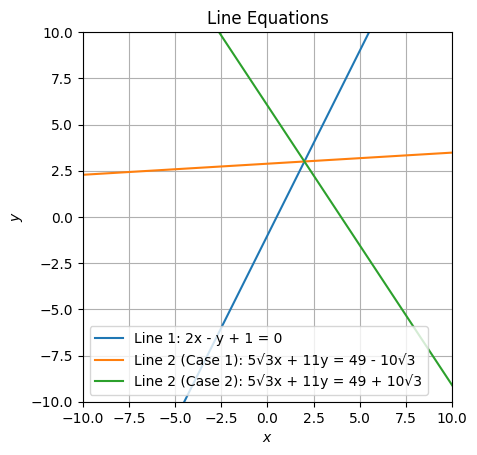
\includegraphics[width=\columnwidth]{line.png}
    \caption{straight line}
    \label{fig:enter-label}
\end{figure}

\end{document}

